\section{Very old notes}
\radu{Notes not touched since 5 June.}

Problem setting in Section~\ref{sec:problem:setting}

Communication cost in Section~\ref{sec:communication:cost}

\subsection{Problem setting}\label{sec:problem:setting}

\subsubsection{Parameters}
We first identify some of the parameters that we have to consider in the problem setting.

\begin{enumerate}
\item The {\em initial format} of the data: (i) standard relational, or (ii) factorized representation.

\item The {\em communication format} between nodes: (i) standard relational, or (ii) factorized representation.

\item The {\em initial location} of the data: (i) centralized in one node, or (ii) distributed in several nodes.
For the moment we decided to reason in terms of only one node because we believe that in the case of several nodes we have just to apply the same reasoning for each node.

\item The {\em heterogeneity} of the nodes (provided that the data is initially factorized and located in different nodes): (i) all nodes use the same f-tree, or (ii) each node uses its own f-tree.
We always assume that the path constraints are given.
The idea is to ensure that when restructuring we do not get a size increase due to the paths that appear in the initial f-tree without corresponding to a path constraint.

\item The {\em number of communication rounds}: (i) sequence of standard shuffles (one join at the time), (ii) hypercube shuffle (hash on all join attributes at once), or (iii) a shuffle on a single attribute, but which permits doing all joins in the respective branch (to investigate the conditions when this is possible).

\item The {\em cost model}: (i) communication cost only, assuming that it dominates the actual computation cost~\cite{AfUl11}, or (ii) both computation and communication cost.

\item The type of bounds on the overlap and communication cost: (i) asymptotic e.g., based on the parameter $s(Q)$, or (ii) practical e.g., strategies based on selectivity estimates as in the standard relational world.
\end{enumerate}
Notice that if we consider standard relational data as both initial format and the communication format between the nodes, the setting reduces to~\cite{AfUl11}.


\subsubsection{A first formalization}\label{sec:formalization}
We consider as input a setting $K=(\S, \P, \E, \H)$ that consists of the following components:
\begin{itemize}
\item The {\em schema} $\S$ that is a set of attributes.
\item The {\em path constraints} $\P$ consisting of sets of attributes $\{A_1,\ldots,A_k\}$ that should appear on the same root-to-leaf path in all valid f-trees.
\item The {\em selectivity estimates} $\E$ consisting of:

\begin{description}
\item[$\vals(A)$] -- the number of unique values of type $A$.
\item[$\avg_A(B)$] -- the average number of $B$-values that can appear in the same tuple with a given $A$-value.
\end{description}
Notice that the above notion is useful only for dependent $A$ and $B$.
Otherwise (i.e., if $A$ and $B$ are independent), then $\avg_A(B) = \vals(B)$.

Additionally, notice that we defined the notion of average such that it is not specific to a given f-tree.
When the f-tree is also given, we know the ancestor-descendant relation for all pairs of dependent attributes, hence we are able to use a more intuitive notation:

\begin{description}
\item[$\avgd_A(B)$] -- the average number of $B$-values that are descendant of a given $A$-value.
\item[$\avgu_A(B)$] -- the average number of $B$-values that are ancestor of a given $A$-value.
\end{description}

\item A set of {\em distinguished attributes} $\H=\{A_1,\ldots,A_n\}\subseteq\S$ that we want to hash.

\end{itemize}
We say that an f-tree $\T$ is {\em compatible} with a setting $K=(\S,\P,\E,\H)$ if $\T$ satisfies the schema $\S$ and the path constraints $\P$.

The main problem of interest is: {\em given a setting and a compatible f-tree, what is the communication cost for hashing the distinguished attributes?}

In Section~\ref{sec:communication:cost}, we investigate this problem from two different approaches.
Until then, we develop some useful tools.


\subsubsection{Estimating the size of an f-representation}\label{sec:compute:estimate}
Given an f-tree $\T$ satisfying a given schema and some given path constraints, we show how to estimate the size of an f-representation over $\T$ that also satisfies some given selectivity estimates (defined as in Section~\ref{sec:formalization}).

Let us first define some auxiliary notions.
Given a non-root node $A$ from an f-tree $\T$, by $\lda_\T(A)$ we denote the {\em lowest dependent ancestor} of $A$ in $\T$ i.e., the lowest node $B$ on the path from the root to $A$ in $\T$ such that $A$ and $B$ occur together in a path constraint.
Notice that $A$ should not be the root of any of the trees in $\T$ (since $\T$ can be in fact a forest of trees).

Moreover, given a node $A$ from an f-tree $\T$, by $\partsize_\T(A)$ we denote the partial estimated size of an f-representation over the f-tree corresponding to the subtree of $\T$ rooted at $A$, depending on the path from the root to $A$.

Then, given an f-tree $\T$ and a node $A$ from $\T$ having $B_1,\ldots, B_m$ as children, $\partsize_\T(A)$ is

\begin{itemize}
\item $\vals(A)\times(\partsize_\T(B_1) + \ldots + \partsize_\T(B_m))$ if $A$ is a root,
\item $\avg_{\lda_{\T}(A)}(A) \times(\partsize_\T(B_1) + \ldots + \partsize_\T(B_m))$ otherwise.
\end{itemize}
Given a setting $K=(\S,\P,\E,\H)$ and a compatible f-tree $\T$ of roots $A_1,\ldots,A_k$, we are now able to estimate the size of an f-representation:
\[
\estsize_K(\T) = \sum_{i=1}^k \partsize_\T(A_i).
\]



\subsection{Communication cost}\label{sec:communication:cost}


\subsubsection{Two approaches}
We see two general approaches for minimizing the costs.

\subsubsection{Restructure locally before shipping data over the network.}

This could make sense when:
\begin{itemize}
\item Data is initially stored in different nodes (if all data is initially in the same node, restructuring it in that node seems rather inefficient).
\end{itemize}

This could have as benefits:
\begin{itemize}
\item There will normally be less overlap when communicating the data (in the particular case of a single join, the communication cost would be precisely the size of the data after restructuring).

\item The communicated data is already prepared for joins i.e., the nodes receiving it would not have to do any new restructuring.

\item If data is not initially stored in the most succinct possible factorization, the local restructuring would reduce its size and hence minimize the communication cost (however this seems rather unlikely).
\end{itemize}

This could have as drawbacks:
\begin{itemize}
\item It may be the case that initially the data is structured in the most succinct way and by restructuring we increase its size and hence the communication cost.
In such a case, we may prefer to ship over the network (with larger overlaps) data in the most succinct representation since this cost would probably dominate the computation cost of restructuring it several times at the reducers.
\end{itemize}

\subsubsection{Keep the same structure and shuffle with potentially large overlaps.}

This could make sense when:
\begin{itemize}
\item Data is initially stored in a single node. 
\item The initial factorization is the most succinct.
\end{itemize}

This could have as benefits:
\begin{itemize}
\item The communication cost depends on the initial factorization, hence even in the presence of large overlaps it would depend on a rather small representation.
\item It is a more general case that makes sense regardless the fact that the initial data is in one or more nodes.
\end{itemize}

This could have as drawbacks:
\begin{itemize}
\item There are intuitively larger overlaps hence the communication cost is not minimized.
\end{itemize}



\subsubsection{Computing the communication cost}


\subsubsection{With restructuring}
To minimize the overlaps, we observe that intuitively the distinguished attributes should occur only as prefixes of paths starting from the root.

More formally, we define the {\em prefix property} as follows: given a setting $K=(\S,\P,\E,\H)$ and a compatible f-tree $\T$, each attribute of $\H$ either (i) is a root in $\T$ or (ii) is a child in $\T$ of another attribute from $\H$.
A similar property has been already established for constant delay enumeration in the presence of aggregation and ordering for factorized databases~\cite{BKOZ13}.

Take a setting $K = (\S, \P, \E, \H)$ and a compatible f-tree $\T$.
We introduce next two different approaches for restructuring $\T$ that attempt to minimize its size.

\begin{enumerate}
\item {\em Exhaustive search}.
Iterate over all f-trees that are compatible with $K$ and satisfy the prefix property.
Choose the one that minimizes the size, let it $\T'$.
Restructure $\T$ until we obtain $\T'$ (using swaps, which also preserve the normalization).

\item {\em Greedy heuristic}.
For each attribute $A\in\H$ that does not satisfy yet the prefix property, compute the estimated size after a sequence of swaps until $A$ satisfies this condition.
Perform these swaps only for the attribute $A$ that minimizes the size.
Iterate this until all attributes in $\H$ satisfy the prefix property.
\end{enumerate}
Notice that for both strategies the notion of size is generic and can be instantiated either with asymptotic size (i.e., based on the parameter $s$) or with the estimated size.
Similar strategies have been already developed in the context of query evaluation in factorized databases~\cite{BaOlZa12}.

Regardless the chosen strategy, assume that the initial $\T$ is now restructured as a $\T'$ that satisfies the prefix property.
To estimate the communication cost, we have to employ the techniques described in Section~\ref{sec:compute:estimate}.

Assume $p$ communication nodes.
Let $B_1,\ldots, B_m$ be the non-distinguished children in $\T'$ of the distinguished attributes.
By construction, there is no distinguished attribute under any of these $B_i$.
The communication cost is:
\[
\estsize_K(\T') + p\times \sum_{i=1}^m\partsize_\T(B_i).
\]
The second part of the above sum corresponds to the overlaps due to the subtrees of distinguished attributes that may be communicated for different combinations of the distinguished ones.

It would be interesting to further refine the above bound by taking into account the actual {\em shares}~\cite{AfUl11} of the distinguished attributes.

Additionally, notice that in the particular case where there is only one distinguished attribute (which should actually be a root in $\T'$), the overlap should be 0.
This does not follow from the above formula, but hopefully it will after we refine it to take into account the actual shares.


\subsubsection{Without restructuring}
If we do not want to restructure, there may be larger overlaps because now there may be non-distinguished attributes $B$ that have distinguished attributes $A$ as descendants.
These additional overlaps concern the parts of the tree that are below $B$ and not below $A$ and which intuitively imply larger overlaps since they are closer to the root.


\begin{example}\label{ex:two:trees}\normalfont
Take the schema $\S=\{A,B,C,D\}$, and the path constraints $\{A,E\}, \{A,B,D\}, \{B,C\}$.
We present in Figure~\ref{fig:two:trees} two valid f-trees.

{\bf Costs based on asymptotic bounds.}
Both f-trees have $s(\T)=2$ hence they could be used to represent the asymptotically smallest f-representations over the given schema and constraints.
We can imagine situations where some of the nodes store factorized data according to $\T_1$ and other nodes store factorized data according to $\T_2$.
Given data structured according to the f-tree $\T_1$ from Figure~\ref{fig:two:trees}, we present in Table~\ref{table:overlaps} the corresponding overlap and communication cost for hashing on each of the attributes.

{\bf Costs based on selectivity estimators.}
Assume that the data is initially structured according to the f-tree $\T_1$ and we want to perform the swap $\chi_{A,B}$ to obtain data structured according to the f-tree $\T_2$.
Assume the following estimates that have been already computed after some preprocessing:
\begin{itemize}
\item $\vals(A)$, $\vals(B)$, $\vals(C)$, $\vals(D)$, $\vals(E)$.
\item For the path constraint $\{A, B, D\}$: $\avgd_A(B)$, $\avgd_A(D)$, $\avgd_B(D)$, $\avgu_B(A)$, $\avgu_D(A)$, $\avgu_D(B)$.
\item For the path constraint $\{A, E\}$: $\avgd_A(E)$, $\avgu_E(A)$.
\item For the path constraint $\{B, C\}$: $\avgd_B(C)$, $\avgu_C(B)$.
\end{itemize}
The size of an f-representation $E_1$ over an f-tree $\T_1$ is:
\[
|E_1| = \vals(A) \times (\avgd_A(B)\times (\avgd_B(C) + \avgd_B(D)) +\avgd_A(E)).
\]
After the swap $\chi_{A,B}$, we obtain the f-representation $E_2$ according to $\T_2$, whose estimated size is:
\[
|E_2| = \vals(B) \times (\avgu_B(A)\times (\avgd_A(E) + \avgd_A(D)) + \avgd_B(C)).
\]
Thus, by hashing the $B$'s, the communication cost $\cc(B)$ is precisely $|E_2|$.

Let us now compute the communication cost without local restructuring, which may imply some overlaps for the $A$'s and $E$'s since the other attributes (i.e., $C$ and $D$) depend on the $B$'s only.

Assume that we have $p$ nodes and we hash on $B$'s i.e., we have a function $h$ that maps the $B$-values to $p$ buckets.
The data sent to a node $n\in\{1,\ldots,p\}$ is basically the initial f-representation from which we have removed all subtrees rooted in $B$-values $b$ such that $h(b)\neq n$.
In such a case, the communication cost for $B$ is:
\[
\cc'(B) = |E_1| + p\times \vals(A)\times \avgd(A,E).
\]
Thus, we prefer local restructuring instead of overlaps if $\cc(B)\leq \cc'(B)$ i.e.,
\begin{flalign*}
&\vals(B) \times (\avgu_B(A)\times (\avgd_A(E) + \avgd_A(D)) + \avgd_B(C)) \leq\\
&~~\leq  \vals(A) \times (\avgd_A(B)\times (\avgd_B(C) + \avgd_B(D)) +\avgd_A(E))+\\
&~~+ p \times \vals(A)\times \avgd_A(E)
\end{flalign*}
which can be furthermore rewritten as
\begin{flalign*}
&\vals(B) \times (\avgu_B(A)\times (\avgd_A(E) + \avgd_A(D)) + \avgd_B(C)) \leq\\
&~~\leq  \vals(A) \times (\avgd_A(B)\times (\avgd_B(C) + \avgd_B(D))+\\
&~~ +(p+1)\times\avgd_A(E))
\end{flalign*}
By fitting the actual estimation values in the above formula, we are able to reason which of the two strategies is preferable in practice.
\qed\end{example}
Intuitively, when the initial $\T_1$ corresponds to the asymptotically the most succinct representation and $s(\T_1)=s(\T_2)$, it may be preferable to restructure because the communication cost will be asymptotically the same as the initial size.
\begin{figure}[t]\centering
\subfigure[F-tree $\T_1$.]{
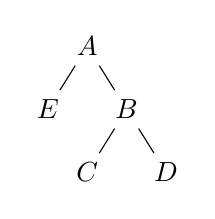
\begin{tikzpicture}[xscale=0.5, yscale=0.8]
\node at (-1, 0) (n1) {$A$};
\node at (-2, -1) (n0) {$E$} edge[-] (n1);
\node at (0, -1) (n2) {$B$} edge[-] (n1);
\node at (-1, -2) (n3) {$C$} edge[-] (n2);
\node at (1, -2) (n4) {$D$} edge[-] (n2);
\end{tikzpicture}
}~~~~~~~~~
\subfigure[F-tree $\T_2$.]{
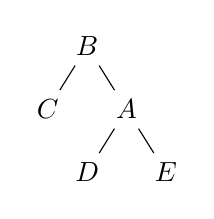
\begin{tikzpicture}[xscale=0.5, yscale=0.8]
\node at (-1, 0) (n1) {$B$};
\node at (-2, -1) (n0) {$C$} edge[-] (n1);
\node at (0, -1) (n2) {$A$} edge[-] (n1);
\node at (-1, -2) (n3) {$D$} edge[-] (n2);
\node at (1, -2) (n4) {$E$} edge[-] (n2);
\end{tikzpicture}
}
\caption{\label{fig:two:trees}F-trees from Example~\ref{ex:two:trees}.}
\end{figure}


\begin{table}[t]\centering
\begin{tabular}{|c||c|c|}\hline
\em Hashed attribute & \em Overlap & \em Communication cost\\\hline\hline
$A$ & $0$ & $O(|D|^2)$\\\hline
$B$ & $O(|D|)$ & $O(|D|^2 + p\times|D|)$\\\hline
$C$ & $O(|D|)$ & $O(|D|^2 + p\times|D|)$\\\hline
$D$ & $O(|D|^2)$ & $O(|D|^2 + p\times|D|^2)$\\\hline
\end{tabular}
\caption{\label{table:overlaps}Asymptotical overlaps and communication cost from Example~\ref{ex:two:trees}.}
\end{table}





